\documentclass[12pt,aspectratio=169]{beamer}

% Input
\usepackage[utf8]{inputenc}
\usepackage[T1]{fontenc}
\usepackage[letterspace=100]{microtype}
\usepackage{upquote}

% Beamer
\usetheme{metropolis}
\usepackage[sfdefault]{FiraSans}
\usepackage{xcolor}
\definecolor{blue}{HTML}{002957}
\definecolor{red}{HTML}{F1563F}
\setbeamercolor{palette primary}{fg=white,bg=blue}
\setbeamercolor{title separator}{fg=red,bg=blue}
\setbeamercolor{frametitle}{fg=white,bg=blue}
\setbeamercolor{progress bar}{fg=red,bg=blue}
\setbeamercolor{alerted text}{fg=red,bg=blue}
\makeatletter
\setlength{\metropolis@titleseparator@linewidth}{2pt}
\setlength{\metropolis@progressonsectionpage@linewidth}{2pt}
\setlength{\metropolis@progressinheadfoot@linewidth}{2pt}
\makeatother

% Graphics
\usepackage{graphicx}
\usepackage{epstopdf}
\DeclareGraphicsExtensions{.png,.pdf,.eps}
\tikzset{
  invisible/.style={opacity=0},
  visible on/.style={alt={#1{}{invisible}}},
  alt/.code args={<#1>#2#3}{%
    \alt<#1>{\pgfkeysalso{#2}}{\pgfkeysalso{#3}} % \pgfkeysalso doesn't change the path
  },
}
\usetikzlibrary{arrows, shapes}

% Various
\usepackage{hyperref}
\usepackage{minted}
\usepackage{fontawesome}
\usepackage{multicol}
\usepackage[normalem]{ulem}

% Title
\title{Pulumi – sovelluspalvelinympäristö koodina}
\subtitle{DIP-konferenssi}
\date{27.03.2024}
\author{Asko Soukka}
\institute{\vspace{1cm}
\includegraphics[height=1.5cm]{images/jyu-vaaka-kaksikielinen.eps}}

\newcommand{\setmytemplate}{}

\newcommand\Wider[2][1cm]{%
\makebox[\linewidth][c]{%
  \begin{minipage}{\dimexpr\textwidth+#1\relax}
  \raggedright#2
  \end{minipage}%
  }%
}

\begin{document}

\setbeamercolor{background canvas}{bg=white}
\setbeamertemplate{footline}{}

%---------------------------------------------------------------------------------------

\setbeamertemplate{footline}[plain]
\setbeamertemplate{background canvas}[default]
\maketitle

%---------------------------------------------------------------------------------------

\section{Infrastructure as Code}

\begin{frame}[fragile]{Terraform language syntax}
\footnotesize
\begin{minted}{hcl}
resource "vsphere_virtual_machine" "vm" {
  name             = "foo"
  resource_pool_id = data.vsphere_compute_cluster.cluster.resource_pool_id
  datastore_id     = data.vsphere_datastore.datastore.id
  num_cpus         = 1
  memory           = 1024
  guest_id         = "other3xLinux64Guest"
  network_interface {
    network_id = data.vsphere_network.network.id
  }
  disk {
    label = "disk0"
    size  = 20
  }
}
\end{minted}
\end{frame}

\begin{frame}
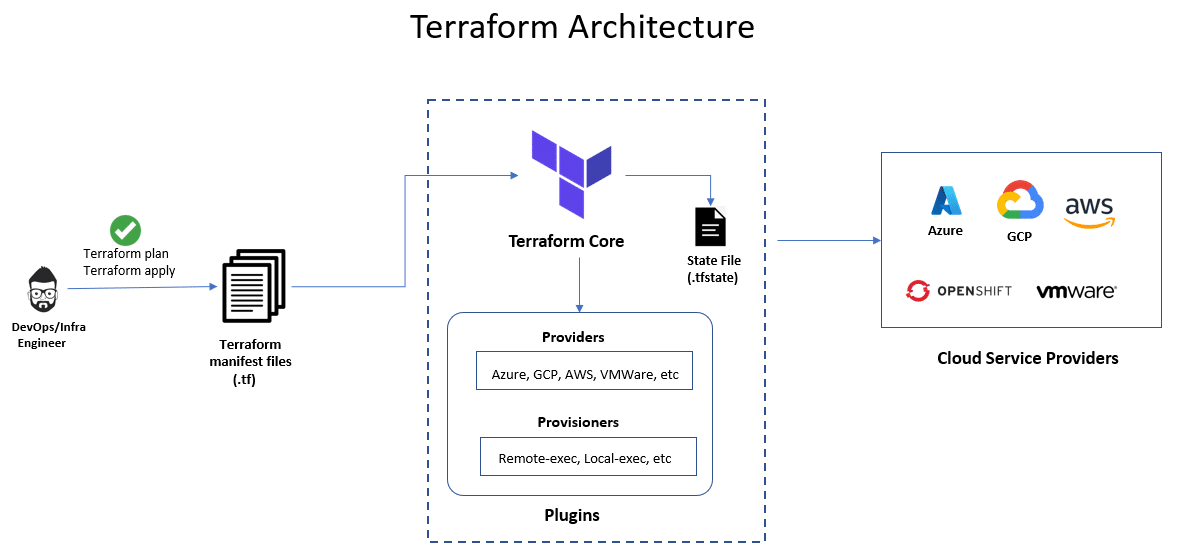
\includegraphics[width=0.8\paperwidth]{pulumi-images/terraform-architecture-diagram.png}
\end{frame}

\section{With Pulumi}

\begin{frame}
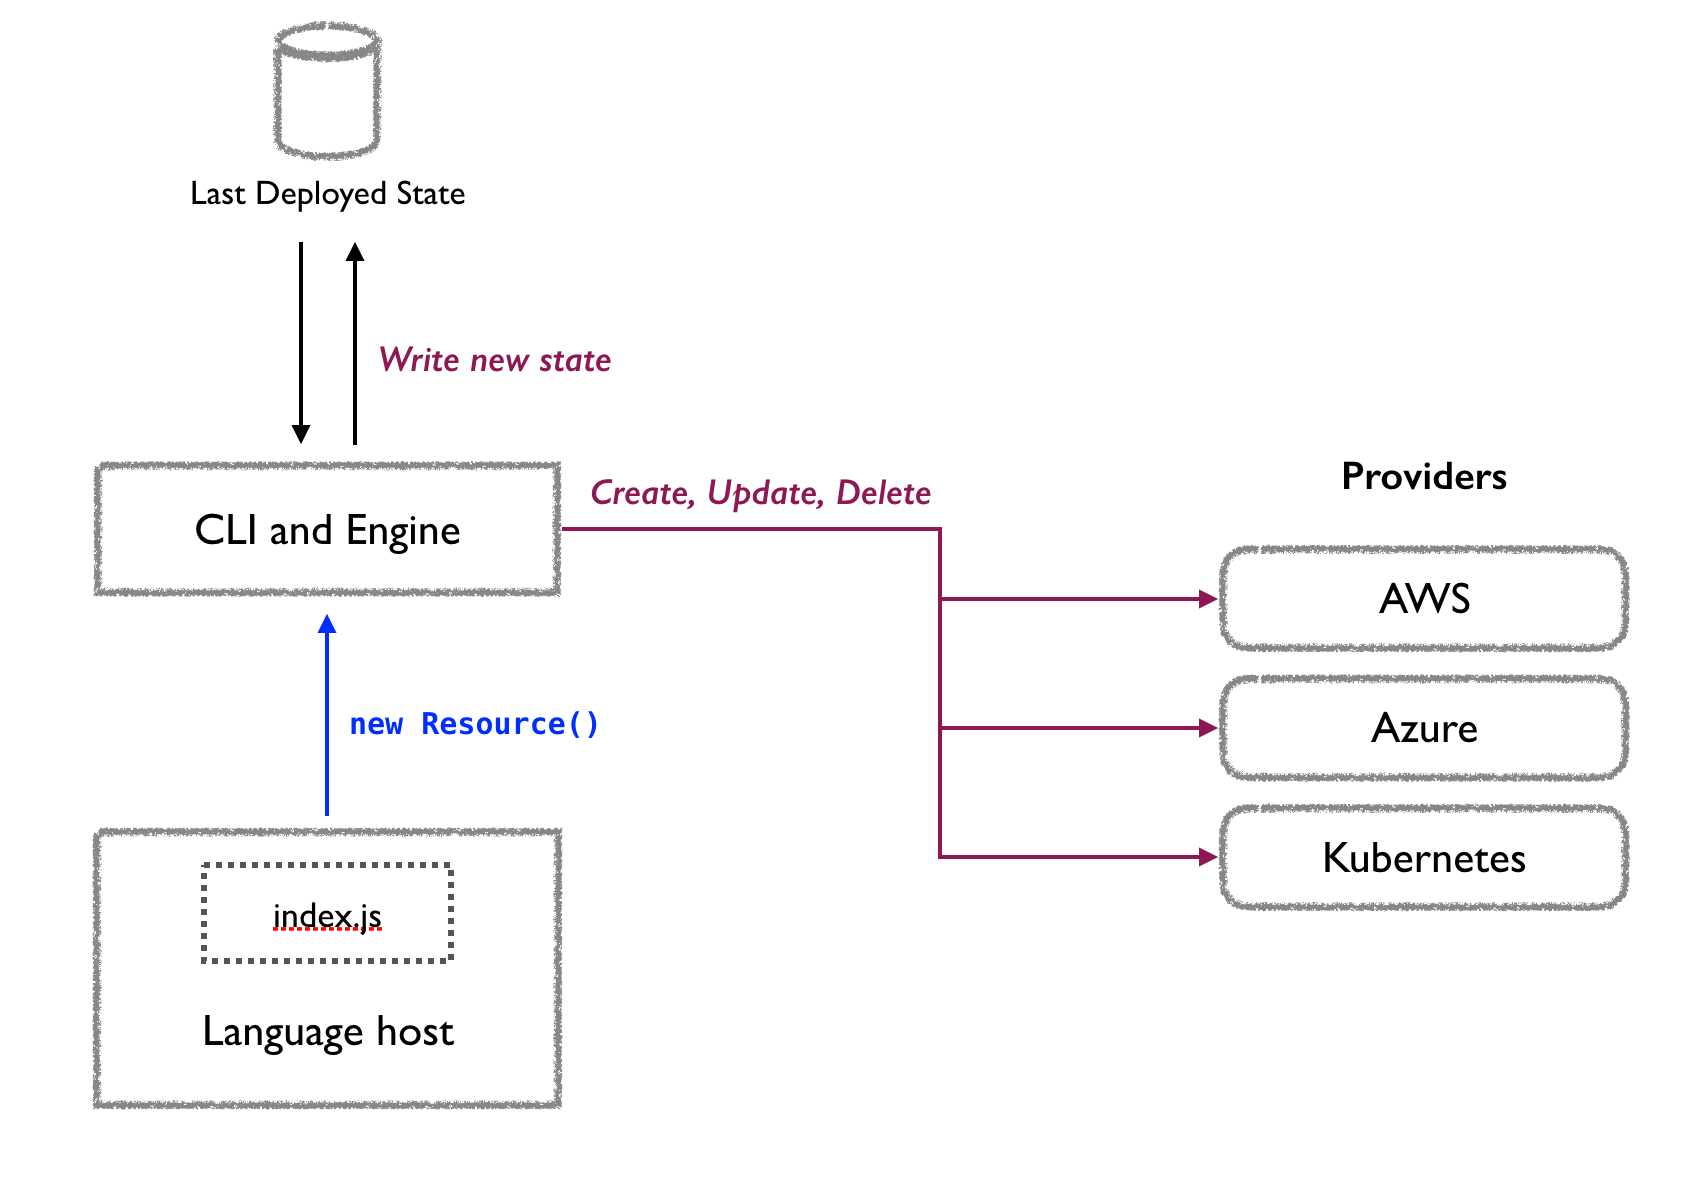
\includegraphics[width=0.8\paperwidth]{pulumi-images/pulumi-architecture-diagram.png}
\end{frame}

\begin{frame}[fragile]{Pulumi resource in Python}
\footnotesize
\begin{minted}{python}
virtual_machine = vsphere.VirtualMachine("vm",
    name="foo",
    resource_pool_id="your_resource_pool_id",
    datastore_id="your_datastore_id",
    num_cpus=1,
    memory=1024,
    guest_id="other3xLinux64Guest",
    network_interfaces=[vsphere.VirtualMachineNetworkInterfaceArgs(
        network_id="your_network_id",
    )],
    disks=[vsphere.VirtualMachineDiskArgs(
        label="disk0",
        size=20,
    )],
)
\end{minted}
\end{frame}

\begin{frame}[fragile]{Pulumi resource in YAML}
\footnotesize
\begin{minted}{yaml}
resources:
  vm:
    type: vsphere:index/virtualMachine:VirtualMachine
    properties:
      name: foo
      resourcePoolId: ${resourcePool.id}
      datastoreId: ${datastore.id}
      numCpus: 1
      memory: 1024
      guestId: other3xLinux64Guest
      networkInterfaces:
        - networkId: ${network.id}
      disks:
        - label: disk0
          size: 20
\end{minted}
\end{frame}

\begin{frame}[fragile]{Pulumi automation API}
\footnotesize
\begin{minted}{python}
### Create and deploy stack with dynamic Pulumi program
pulumi.automation.create_or_select_stack(
    stack_name="test",
    project_name="proxy",
    program=..,
    opts=pulumi.automation.localworkspaceoptions(
        project_settings=pulumi.automation.projectsettings(
            name="proxy"
            runtime="python",
            backend=...
        ),
        secrets_provider=...
    ),
).up() ### Go!
\end{minted}
\end{frame}

\begin{frame}[fragile]{Accessing asynchronous outputs}
\footnotesize
\begin{minted}{python}
### Define any resource
secret_id = vault.approle.AuthBackendRoleSecretId(
    f"{approle.name}:{machine.name}",
    role_name=approle.name,
    with_wrapped_accessor=True,
    wrapping_ttl="24h",
)
\end{minted}
\begin{minted}{python}
### Use future to access and use output when available
pulumi.export(
    f"approle:{approle.name}:{machine.name}:state",
    secret_id.wrapping_accessor.apply(lambda accessor: ...)
)
\end{minted}
\end{frame}

\begin{frame}[fragile]{Accessing previous state}
\footnotesize
\begin{minted}{python}
### Retrieve previous state with dummy program
state = pulumi.automation.create_or_select_stack(
    program=lambda: None,
    ...
).export_stack()
\end{minted}
\begin{minted}{python}
### Final stack with real program and previous staet
stack = pulumi.automation.create_or_select_stack(
    program=create_program(state),
    ...
)
\end{minted}
\begin{minted}{python}
### ...
stack.up()
\end{minted}
\end{frame}

\section{MVRE \& Pulumi}

\begin{frame}[fragile]{MVRE NixOS configuration}
\footnotesize
\begin{minted}{nix}
{ config, ... }: {
  imports = [ ./miniotest0.nix ];

  fileSystems."/var/persist".device = "/dev/disk/by-uuid/...";
  fileSystems."/var/lib/minio".device = "/dev/disk/by-uuid/...";

  networking.hostName = "mvre-miniotest1";
  networking.interfaces."intraserv-2" = {
    ipv4.addresses = [{ address = "..."; prefixLength = 23; }];
    macAddress = "...";
  };

  services.udev.extraRules = ''
    ACTION=="add", SUBSYSTEM=="net", ATTR{address}=="${config.networking.interfaces.intraserv-2.macAddress}", NAME="intraserv-2"
  '';
}
\end{minted}
\end{frame}

\begin{frame}[fragile]{MVRE Nix to Pulumi mapping}
\footnotesize
\begin{minted}{toml}
[minio.test]
disks = [
    { name = "miniotest1./", datastore = "mvre_01_200" },
    { name = "miniotest2./", datastore = "mvre_01_200" },
    { name = "miniotest3./", datastore = "mvre_02_201" },
    { name = "miniotest4./", datastore = "mvre_02_201" },
]
machines = [
    { name = "miniotest1", datastore = "mvre_01_200", host = "aatos-l40s.cc.jyu.fi" },
    { name = "miniotest2", datastore = "mvre_01_200", host = "erkko-l40s.cc.jyu.fi" },
    { name = "miniotest3", datastore = "mvre_02_201", host = "jane-a30.cc.jyu.fi" },
    { name = "miniotest4", datastore = "mvre_02_201", host = "jane-a30.cc.jyu.fi" },
]
\end{minted}
\end{frame}

\begin{frame}[fragile]{MVRE Pulumi CLI}
\footnotesize
\begin{minted}{shell}
Usage: mvre.py [OPTIONS] PULUMI_PROJECT PULUMI_STACK COMMAND [ARGS]...

  MVRE Pulumi CLI

Options:
  --preview  Require confirmation before proceeding.
  --cancel   Cancel Pulumi lock on stack.
  --help     Show this message and exit.

Commands:
  down
  up
\end{minted}
\end{frame}

\begin{frame}[fragile]{MVRE Pulumi Program}
\footnotesize
\begin{minted}{python}
def create_pulumi_program(
    project: ProjectStack,
    catalog: FlakeCatalog,
    vault_addr: str,
) -> None:
    disks: Dict[str, vsphere.File] = {}

    for disk in project.disks:
        disks[resource_name(disk.name)] = vsphere_file(disk, catalog)

    for machine in project.machines:
        vsphere_virtual_machine(machine, catalog, vault_addr, disks)
\end{minted}
\end{frame}

%---------------------------------------------------------------------------------------

\begin{frame}[standout]
\vfill

\includegraphics[height=0.50\paperheight]{pulumi-images/nixos-logo-white-hires.png}
\end{frame}

%---------------------------------------------------------------------------------------


\end{document}
